\section{Introduction}\label{introduction}

\subsection{Motivation}\label{motivation}

The work done in this report is done in cooperation with Sensomar SEALAB.
Sensomar SEALAB is a company developing camera systems for underwater use. Most of SEALABs technology is planned for use in the fishing industry, especially aimed towards salmon breeding industry. 

The aquaculture industry has grown dramatically over the last decades, and the fishing industry has become more and more industrial. This industrialisation of fish breeding has made the production more profitable, but it has also caused the concentration of salmon lice to grow dramatically. With the use of good camera systems along with the right image processing it can be possible to detect the lice much earlier than now. 

Another challenge for the fish breeding companies is estimation of biomass. A grown salmons weight can vary from around two to ten kilos. This makes it hard for the companies to know the volume of fish they have in their cages at any time, and difficult to know how much fish they can sell. If they sell more fish then the cage contains they need to purchase fish from competitors at a steep price. The biomass estimation directly effects the profit, therefore, providing a solution for biomass estimation would very much benefit the companies. 

SEALABs current goal is to develop an advanced underwater camera system that can both detect salmon lice and measure biomass in the fish cages.
The system currently used by SEALAB for the biomass estimation is the Raytrix R42 camera, a light field camera computing both 2D and 3D images with corresponding depth data in one frame. The camera is the best in its field. Features for the Raytrix R42 camera is explained is section \ref{the_raytrix_camera}. 
The depthmap produced by the cameras software can be used to estimate the volume of an object. Depthmaps computed by the Raytrix is very accurate in air, but underwater, the depthmap is not as accurate. Reasons for this inaccuracy can come directly from the water mediums properties, it can depend on the lightning, the background and/or particles in the water. This means that even though the best available camera technology is used, the results directly is still not good enough for correct volume measurement.

With the use of image processing for noise and particle removal, together with testing of different lightning and background conditions, it is reasonable to believe that the estimates for biomass of fish could be improved.

This report shows the exploration of different processing possibilities done on data extracted from the Raytrix R42. Different testing conditions is explored, and a suggested solution is provided and tested.


%%%%%%%%%%%%%%%%%%%%%%%%%%%%%%%%%%%%%%%%%%%%%%%%%%%%%%%%%%%%%%%%%%%%%%


\subsection{Report Outline} \label{report_outline}

First, section \ref{overview} describes the different approaches useful for solving the problem at hand. Next, the aim for this report is explained in section \ref{aim of study}, and the implementation of the presented solution is described in \ref{methods and implementation}, along with different tests. Results is presented in section \ref{results}, and section \ref{conclusion} describes to what degree the problem is solved. All code is provided, and suggestions for further work are given at the end of the paper.

All image processing done throughout this project is done through the use of C++ and OpenCV library. Provided results with 3D images is made in MATLAB.


%%%%%%%%%%%%%%%%%%%%%%%%%%%%%%%%%%%%%%%%%%%%%%%%%%%%%%%%%%%%%%%%%%%%%%

\subsection{The Raytrix Camera}\label{the_raytrix_camera}

\begin{figure}[ht]
    \centering
    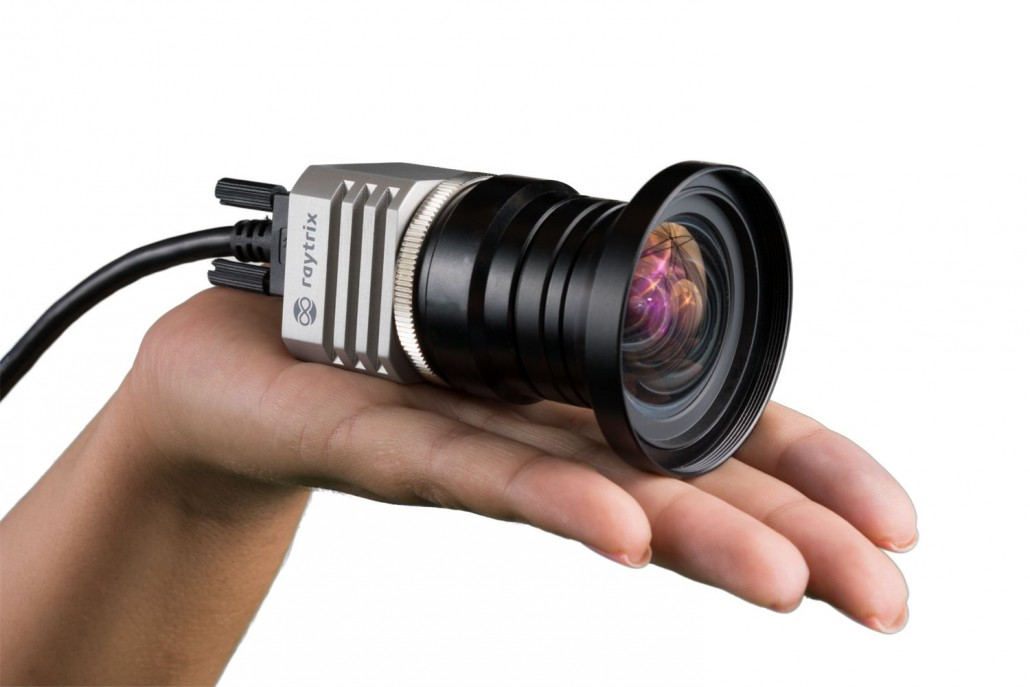
\includegraphics[width=.9\linewidth]{images/introduction/raytrix_camera}
    \caption{Raytrix R42 Camera}
    \label{fig:raytrix_camera}
\end{figure}

The camera used throughout this project is the Raytrix R42 camera. The camera is developed by Raytrix, a German company which offers several 3D Light Field cameras intended for professional and industrial use. The R42 is their highest resolving light field camera to date. It is based on a 42 megaray sensor and offers an effective resolution up to 10 megapixels at 7 FPS. \cite{website:raytrix_r42}

Light Field cameras are a new type of 3D-cameras that capture a standard image together with the depth information of a scene. Metric 3D information can be captured with a single light field camera through a single lens in a single shot using just the available light. Raytrix has specialized on developing light field cameras for industrial applications. A patented micro lens array design allows for an optimal compromise between high effective resolution and large depth of field. Raytrix cameras are already in use in applications like volumetric velocimetry, plant phenotyping, automated optical inspection and microscopy, to name a few. \cite{website:raytrix_main}

This camera is therefore very useful for industrial purposes, as you can get both a clear image, a depth map, and a 3D model of the scene. It has though no documented use underwater, and since the physical properties of water cause degradation effects not present in air, the depth measurements get affected. We get both "holes" in the object, and detected particles in front of the object. If we are going to use this camera technology to measure volume of fish, we need to improve the data received from the camera. Particles in front of the fish needs to be removed, and holes in the fish filled.

The Raytrix camera is build up by a main lens in front, a micro lens array, and the image sensor behind. The micro lens array has many thousand micro lenses, 4000x2600 lenses. The micro lens array is placed in front of the image sensor inside the camera, which turns the image sensor into a micro-camera array (\ref{fig:light_field}), where each micro-camera sees part of the intermediate image from a slightly different perspective. That is, instead of using a large camera array that looks at the object directly, we can choose a main lens to select the desired field-of-view and create the intermediate image in front of the micro camera array. The images generated by the camera in this setup are processed on a PC with appropriate software algorithms to calculate the scene depth and to reconstruct a 2D image. When all processing is done on a GPU, it allows for 30 megapixel 2D and 3D images per second (30 FPS). \cite{website:raytrix_technology}

\begin{figure}[h]
    \centering
    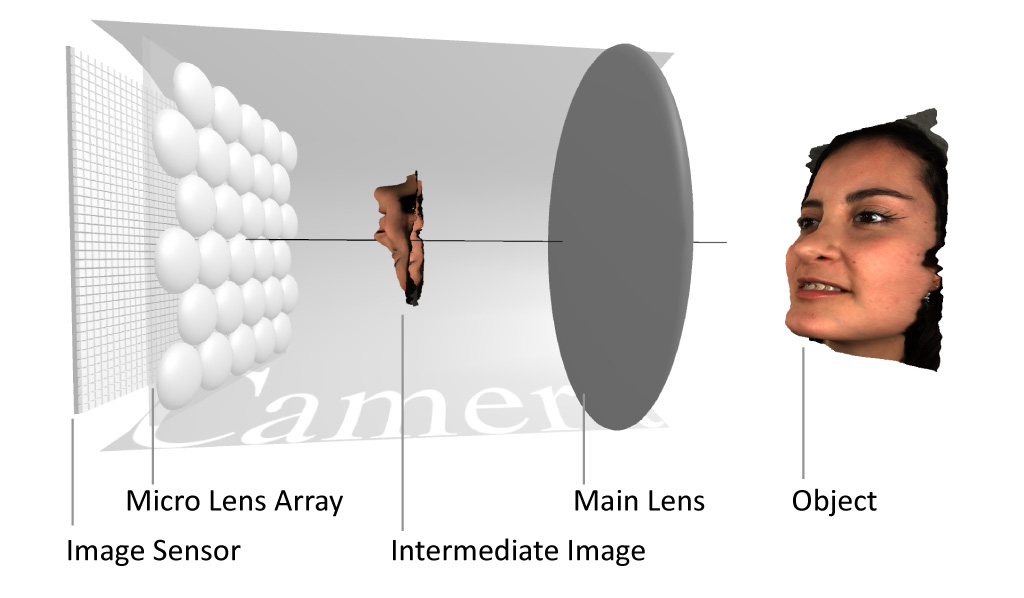
\includegraphics[width=.9\linewidth]{images/introduction/Light-Field-Camera-Schematic}
    \caption{Raytrix Light Field Technology}
    \label{fig:light_field}
\end{figure}

When calibrating the camera the raw image is used to make sure the main objects edges are shown in several of the micro lenses. The more micro lenses picking up one object, the better the depth measurement. 

The raw image shows the capture from all micro lenses, as seen in figure \ref{fig:raw_image}. The camera perform no processing internally, it simply deliver a raw image to a PC, which is then processed on a GPU to obtain the 2D and 3D data. 
The totalfocus image - which is just a normal color image - is made from the raw image on a computer, figure \ref{fig:totalfocus}. 
The depthmap, figure \ref{fig:depthmap}, is computed from the raw image, and the 3D image, figure \ref{fig:3d_image}, is made from the depthmap and the totalfocus image. 
The depth in the depthmap is represented by colors, where red is close to the camera, yellow and green is the object centered during calibration, blue is behind the object, and black has no depth. This means that the optimal depthmap image would be all black, with a yellow and green fish.

\begin{figure}[h]
    \centering
    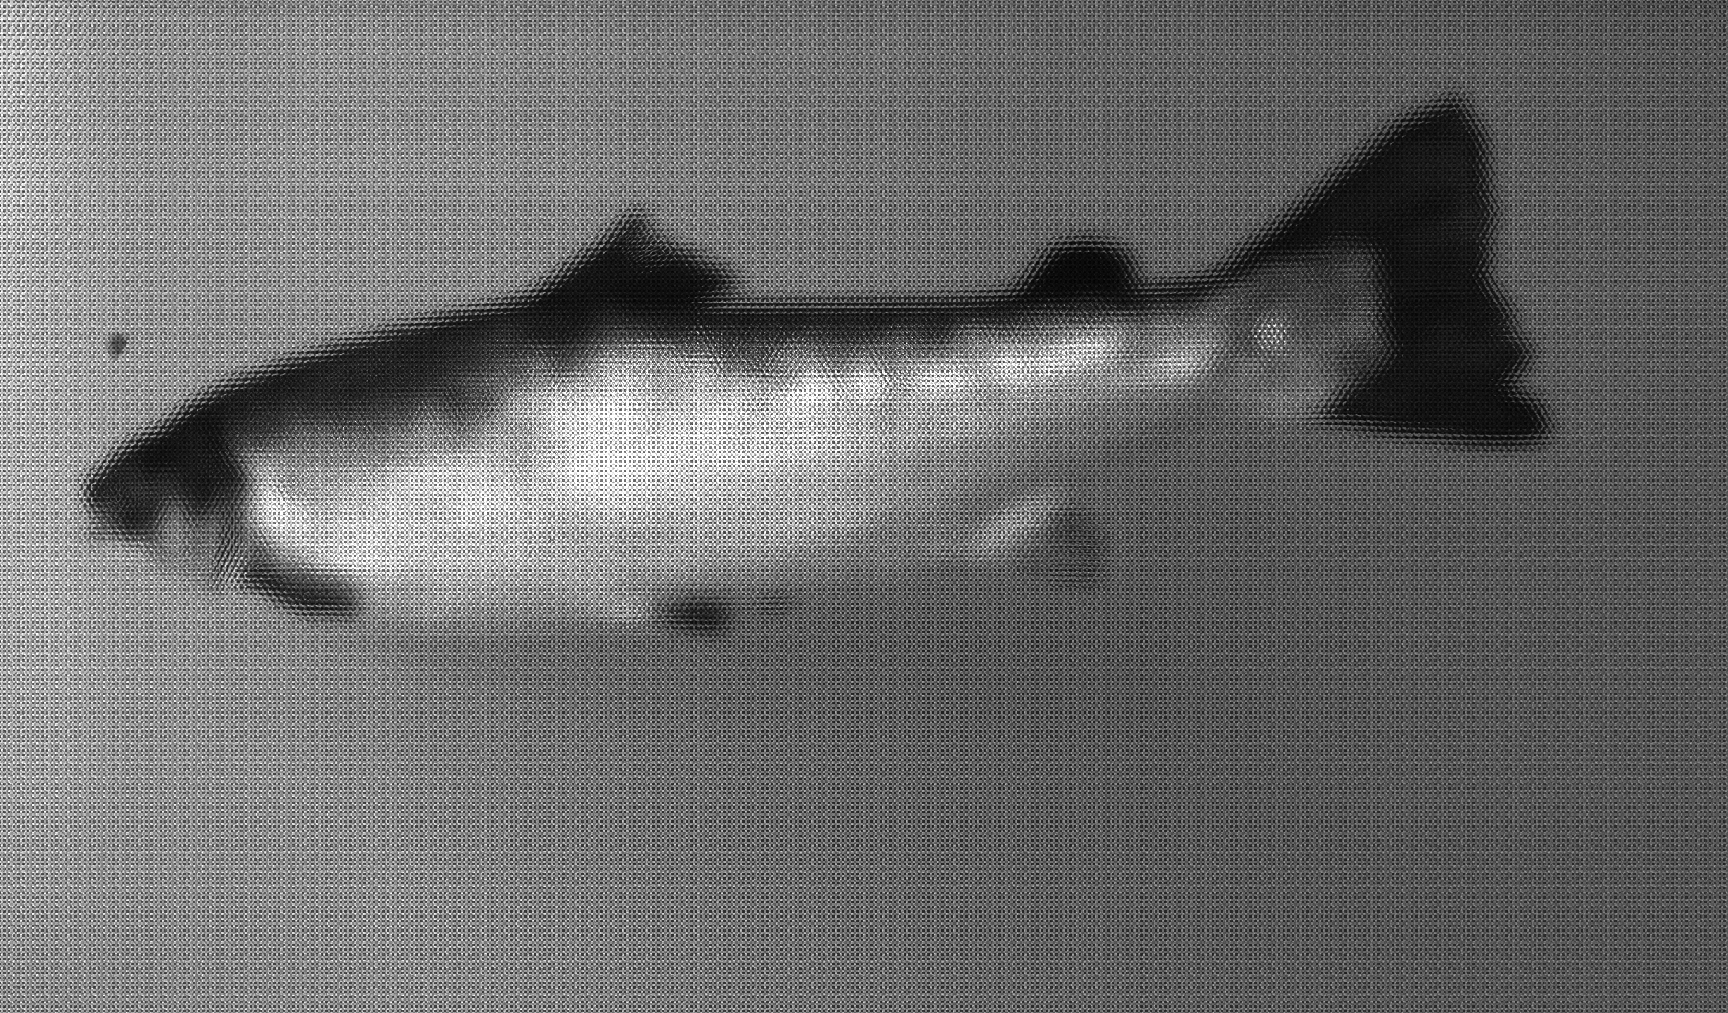
\includegraphics[width=.9\linewidth]{images/introduction/raw}
    \caption{Raw image}
    \label{fig:raw_image}
\end{figure}

\begin{figure}[h]
    \centering
    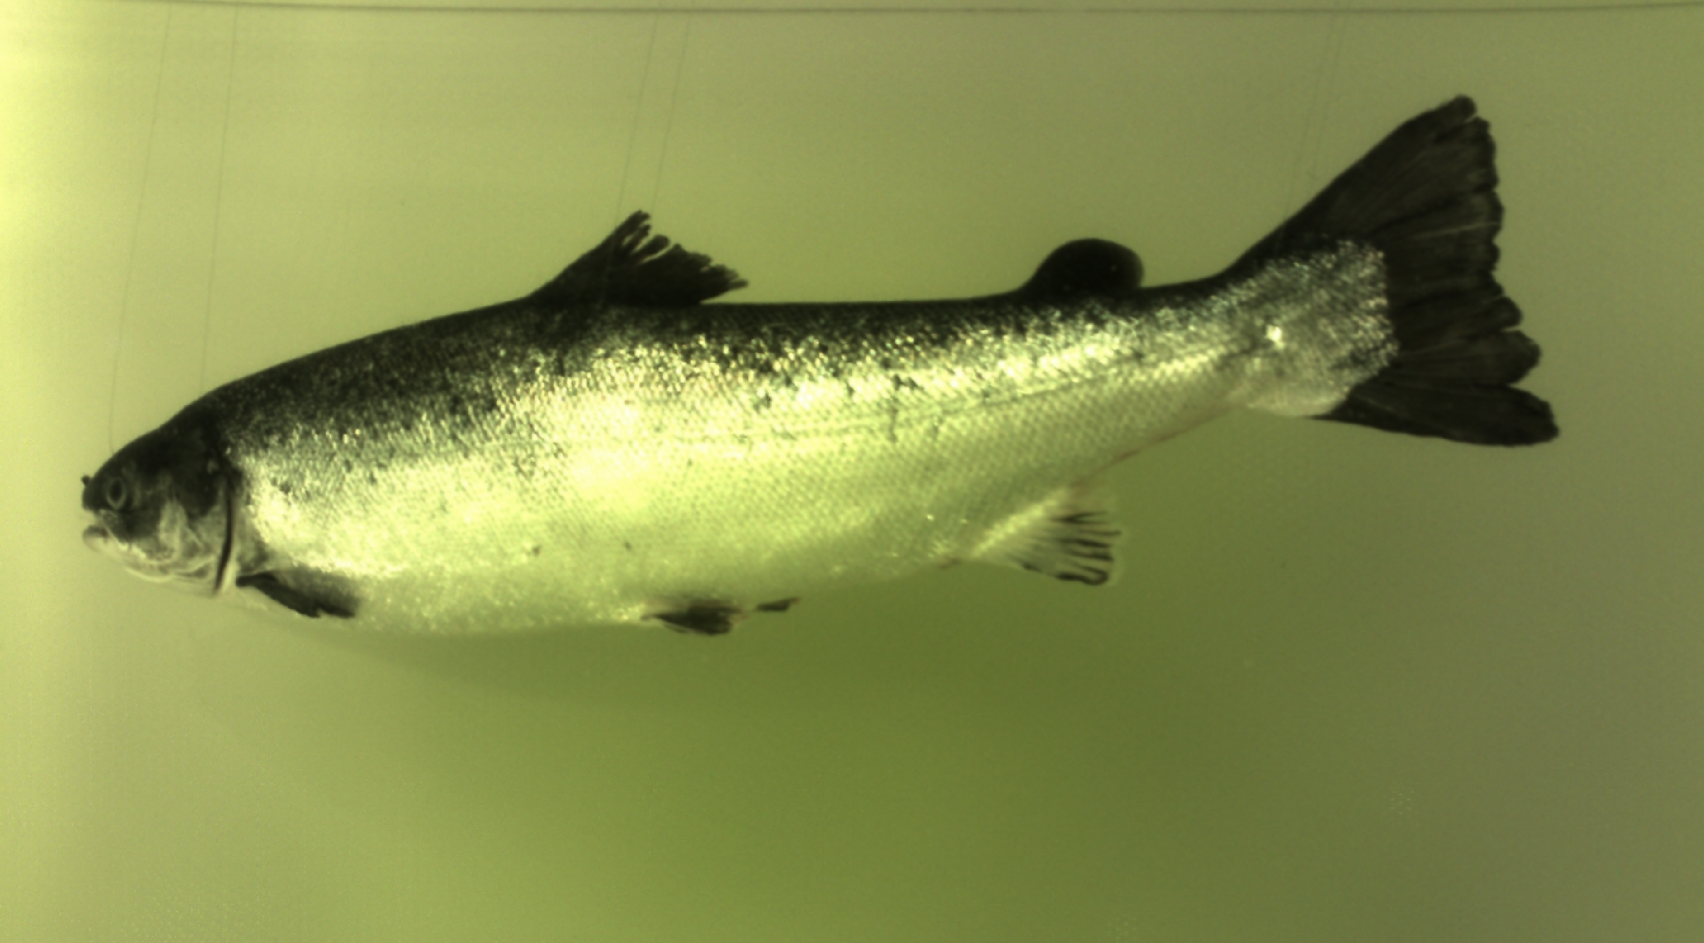
\includegraphics[width=.9\linewidth]{images/introduction/totalfocus}
    \caption{Totalfocus image}
    \label{fig:totalfocus}
\end{figure}

\begin{figure}[h]
    \centering
    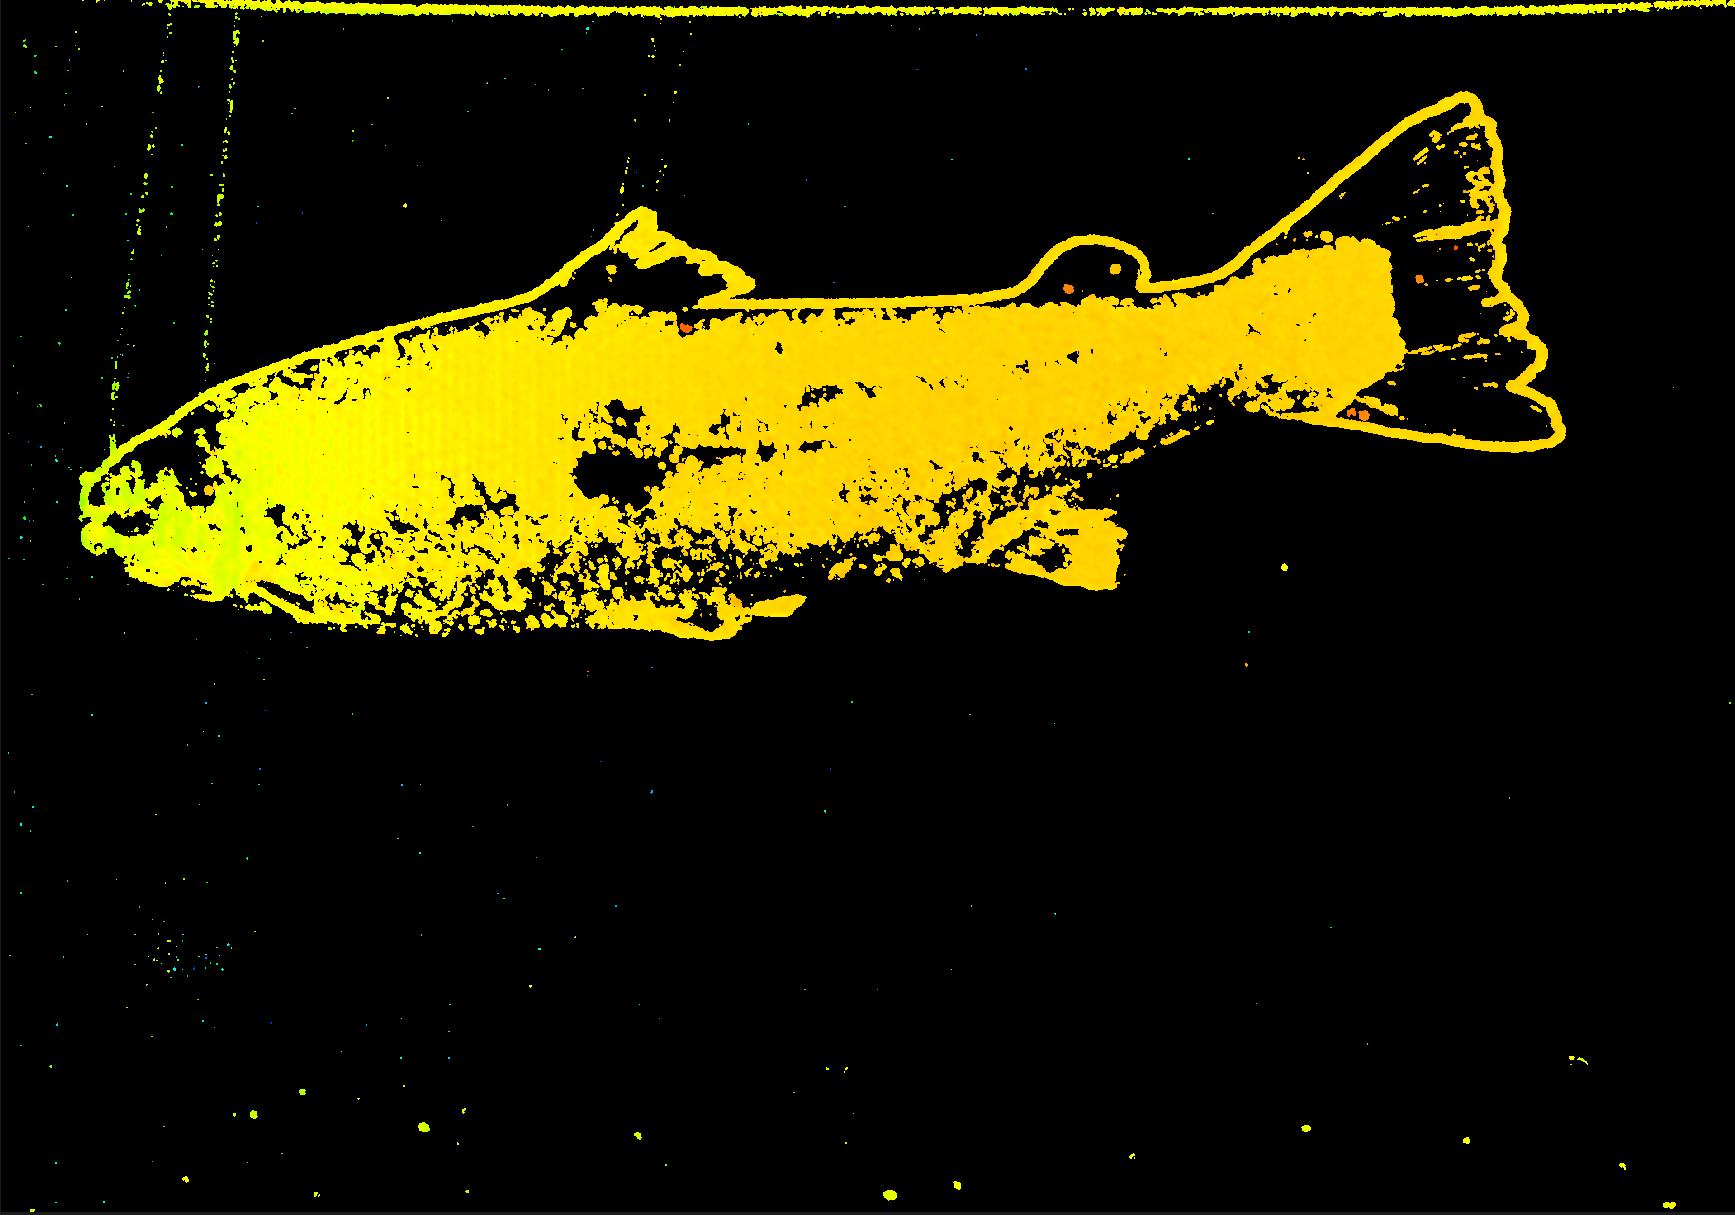
\includegraphics[width=.9\linewidth]{images/introduction/depthmap}
    \caption{Depthmap image}
    \label{fig:depthmap}
\end{figure}

\begin{figure}[h]
    \centering
    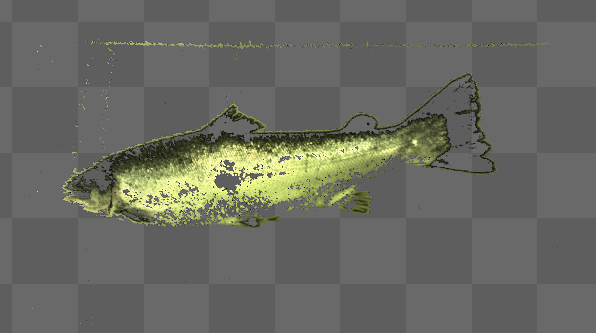
\includegraphics[width=.9\linewidth]{images/introduction/depth3D}
    \caption{3D image}
    \label{fig:3d_image}
\end{figure}

As seen from the 3D image produced in the Raytrix Software, the particles in front will affect the surface of the fish. The same goes for the holes in the fish. What is wanted is a smooth surface of the fish, so that measurements of length, height and thickness is most accurate. Figure \ref{fig:3d_image_side} shows the 3D image in figure \ref{fig:3d_image} turned about 45 degrees to the side. This shows how inaccurate the current 3D model for underwater images are. 
One problem working with the depthmap is that they have their own .ray format. It is not yet possible to do direct image processing using OpenCV on this format, so we therefore convert the depthmap to .png before starting to work on the enhancement.

\begin{figure}[h]
    \centering
    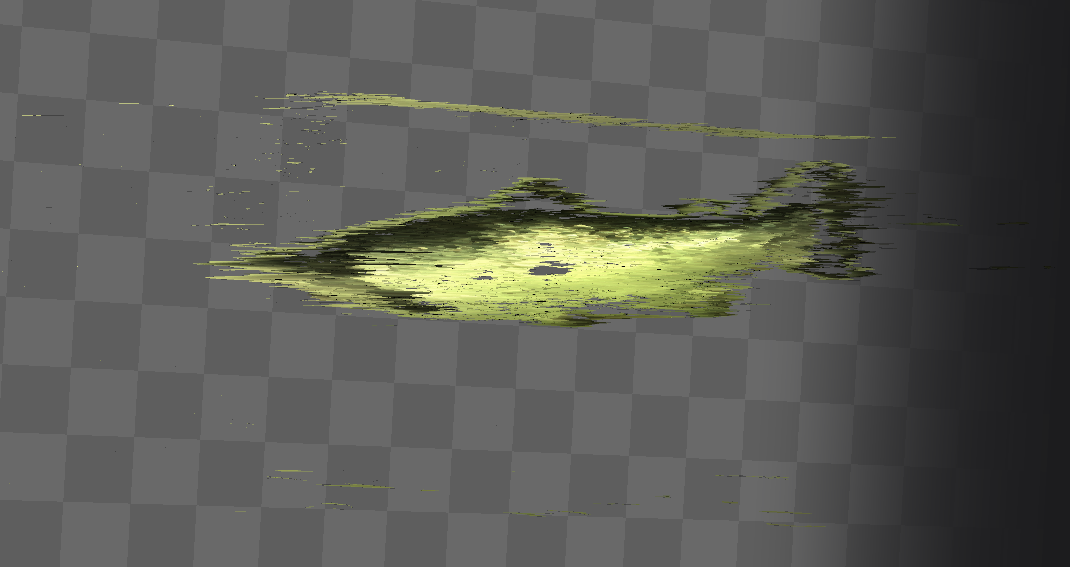
\includegraphics[width=.9\linewidth]{images/introduction/depth3D_side}
    \caption{3D image from the side}
    \label{fig:3d_image_side}
\end{figure}

The reason the Raytrix R42 camera is used by Sensomar SEALAB, is because of its high resolution and high frame-rate. All competitors of Raytrix does not have as good frame-rate and resolution. The Raytrix camera is also different from other light field cameras because it has the light ray crossing behind the micro lens array, while other light field cameras have the light crossing in front of the micro lens array.

All images in this subsection is made with the Raytrix software, RxLive 4.0.

{\color{red}Explain more about how the Raytrix measures depth?? Explain the calibration and the RAW image?? And about Light Field Cameras?}


%%%%%%%%%%%%%%%%%%%%%%%%%%%%%%%%%%%%%%%%%%%%%%%%%%%%%%%%%%%%%%%%%%%%%%


\subsection{The Wetlab}\label{wetlab}

SEALAB has its own test facilities where they have the complete camera setup in a small pool. Aquaculture companies deliver fish for testing.